% Coupon collector with n = 50 coupons: exact law of the number T of draws needed (computed by a recursion), its mean n H_n = 225 and the tail bound point n ln n + 2n. Generated by a short script.
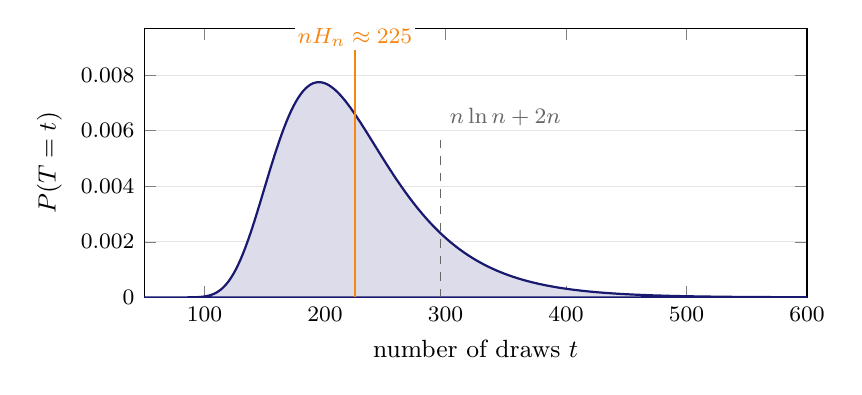
\begin{tikzpicture}
\begin{axis}[width=10cm,height=5cm,xmin=50,xmax=600,ymin=0,ymax=0.00969,xlabel={number of draws $t$},ylabel={$P(T=t)$},
  tick label style={font=\footnotesize},label style={font=\small},scaled y ticks=false,yticklabel style={/pgf/number format/fixed,/pgf/number format/precision=3},ymajorgrids,grid style={black!10}]
\addplot[MidnightBlue,thick,fill=MidnightBlue!15] coordinates {(50,0) (50,0.000000) (52,0.000000) (54,0.000000) (56,0.000000) (58,0.000000) (60,0.000000) (62,0.000000) (64,0.000000) (66,0.000000) (68,0.000000) (70,0.000000) (72,0.000000) (74,0.000000) (76,0.000000) (78,0.000000) (80,0.000000) (82,0.000000) (84,0.000001) (86,0.000001) (88,0.000002) (90,0.000003) (92,0.000006) (94,0.000009) (96,0.000015) (98,0.000022) (100,0.000033) (102,0.000049) (104,0.000069) (106,0.000096) (108,0.000131) (110,0.000175) (112,0.000229) (114,0.000295) (116,0.000375) (118,0.000468) (120,0.000577) (122,0.000702) (124,0.000843) (126,0.001001) (128,0.001176) (130,0.001368) (132,0.001576) (134,0.001799) (136,0.002037) (138,0.002287) (140,0.002548) (142,0.002819) (144,0.003097) (146,0.003381) (148,0.003669) (150,0.003958) (152,0.004247) (154,0.004534) (156,0.004816) (158,0.005091) (160,0.005359) (162,0.005617) (164,0.005864) (166,0.006099) (168,0.006320) (170,0.006527) (172,0.006718) (174,0.006894) (176,0.007054) (178,0.007197) (180,0.007323) (182,0.007432) (184,0.007525) (186,0.007601) (188,0.007661) (190,0.007705) (192,0.007733) (194,0.007747) (196,0.007747) (198,0.007734) (200,0.007707) (202,0.007668) (204,0.007618) (206,0.007557) (208,0.007487) (210,0.007407) (212,0.007319) (214,0.007223) (216,0.007120) (218,0.007011) (220,0.006896) (222,0.006776) (224,0.006652) (226,0.006524) (228,0.006393) (230,0.006259) (232,0.006123) (234,0.005986) (236,0.005847) (238,0.005707) (240,0.005567) (242,0.005427) (244,0.005287) (246,0.005148) (248,0.005009) (250,0.004871) (252,0.004735) (254,0.004601) (256,0.004468) (258,0.004336) (260,0.004207) (262,0.004080) (264,0.003956) (266,0.003833) (268,0.003713) (270,0.003596) (272,0.003481) (274,0.003368) (276,0.003258) (278,0.003151) (280,0.003047) (282,0.002945) (284,0.002846) (286,0.002749) (288,0.002655) (290,0.002564) (292,0.002475) (294,0.002389) (296,0.002305) (298,0.002224) (300,0.002146) (302,0.002069) (304,0.001995) (306,0.001924) (308,0.001855) (310,0.001788) (312,0.001723) (314,0.001660) (316,0.001599) (318,0.001540) (320,0.001484) (322,0.001429) (324,0.001376) (326,0.001325) (328,0.001276) (330,0.001228) (332,0.001182) (334,0.001138) (336,0.001095) (338,0.001054) (340,0.001014) (342,0.000975) (344,0.000939) (346,0.000903) (348,0.000869) (350,0.000835) (352,0.000804) (354,0.000773) (356,0.000743) (358,0.000715) (360,0.000687) (362,0.000661) (364,0.000635) (366,0.000611) (368,0.000587) (370,0.000565) (372,0.000543) (374,0.000522) (376,0.000502) (378,0.000482) (380,0.000464) (382,0.000446) (384,0.000428) (386,0.000412) (388,0.000396) (390,0.000380) (392,0.000365) (394,0.000351) (396,0.000337) (398,0.000324) (400,0.000312) (402,0.000299) (404,0.000288) (406,0.000276) (408,0.000266) (410,0.000255) (412,0.000245) (414,0.000236) (416,0.000226) (418,0.000217) (420,0.000209) (422,0.000201) (424,0.000193) (426,0.000185) (428,0.000178) (430,0.000171) (432,0.000164) (434,0.000158) (436,0.000152) (438,0.000146) (440,0.000140) (442,0.000134) (444,0.000129) (446,0.000124) (448,0.000119) (450,0.000114) (452,0.000110) (454,0.000106) (456,0.000101) (458,0.000097) (460,0.000094) (462,0.000090) (464,0.000086) (466,0.000083) (468,0.000080) (470,0.000077) (472,0.000073) (474,0.000071) (476,0.000068) (478,0.000065) (480,0.000063) (482,0.000060) (484,0.000058) (486,0.000055) (488,0.000053) (490,0.000051) (492,0.000049) (494,0.000047) (496,0.000045) (498,0.000044) (500,0.000042) (502,0.000040) (504,0.000039) (506,0.000037) (508,0.000036) (510,0.000034) (512,0.000033) (514,0.000032) (516,0.000030) (518,0.000029) (520,0.000028) (522,0.000027) (524,0.000026) (526,0.000025) (528,0.000024) (530,0.000023) (532,0.000022) (534,0.000021) (536,0.000020) (538,0.000019) (540,0.000019) (542,0.000018) (544,0.000017) (546,0.000017) (548,0.000016) (550,0.000015) (552,0.000015) (554,0.000014) (556,0.000013) (558,0.000013) (560,0.000012) (562,0.000012) (564,0.000011) (566,0.000011) (568,0.000011) (570,0.000010) (572,0.000010) (574,0.000009) (576,0.000009) (578,0.000009) (580,0.000008) (582,0.000008) (584,0.000008) (586,0.000007) (588,0.000007) (590,0.000007) (592,0.000007) (594,0.000006) (596,0.000006) (598,0.000006) (600,0.000006) (600,0)} \closedcycle;
\draw[BurntOrange,thick] (axis cs:224.96,0)--(axis cs:224.96,0.00891) node[above,font=\footnotesize,fill=white,inner sep=1pt] {$nH_n\approx225$};
\draw[black!60,dashed] (axis cs:295.60,0)--(axis cs:295.60,0.00581) node[above right,font=\footnotesize,align=left] {$n\ln n+2n$};
\end{axis}
\end{tikzpicture}
